\chapter{线虫的特征提取和急性氧化应激实验}
\section{引言}
	在前面的章节中,本文已经介绍了线性梯度稀释芯片的设计以及线虫前景轮廓的分割与单线虫轮廓的解析。
	本章我们将首先介绍线虫轮廓的跟踪,然后介绍基于线虫轮廓跟踪的结果计算线虫的摆动频率特征。最后,通过运用
	本文提出的软硬件系统研究不同线性浓度双氧水对线虫摆动频率的影响,从而验证了本文提出的软硬件平台在高通量自动化药物筛选
	方面具有一定的优势。
\section{线虫轮廓的跟踪}
	由于线虫通体透明,跟踪起来比较困难,本文采用了一种简单有效的跟踪策略。首先经过
	线虫前景轮廓提取和线虫轮廓解析等步骤后,可以得到每一帧图像里所有线虫的轮廓。由
	公式\ref{eq:m}和公式\ref{eq:xy}可以计算出轮廓的重心坐标。
	\begin{equation}
		m_{ji}=\sum_{x,y}I_{x,y}x^iy^j \label{eq:m}
	\end{equation}
	\begin{equation}
		\vec{x}=\frac{m_{10}}{m_{00}},\quad \vec{y}=\frac{m_{01}}{m_{00}}\label{eq:xy}
	\end{equation}
	假设当前帧有n个轮廓,上一帧
	图像有m个轮廓,由每个轮廓的重心坐标可以得到一个$n\times m$的距离矩阵用公式\ref{eq:matrix}
	表示。
		\begin{equation}
                        D=\left[
                \begin{matrix}
                 d_{11}      & d_{12}      & \cdots & d_{1m}      \\
                 d_{21}      & d_{22}      & \cdots & d_{2m}      \\
                 \vdots & \vdots & \ddots & \vdots \\
                 d_{n1}      & d_{n2}      & \cdots & d_{nm}      \\
                \end{matrix}
                \right]\label{eq:matrix}
    \end{equation}
	\begin{figure}[t]
	  \centering
	  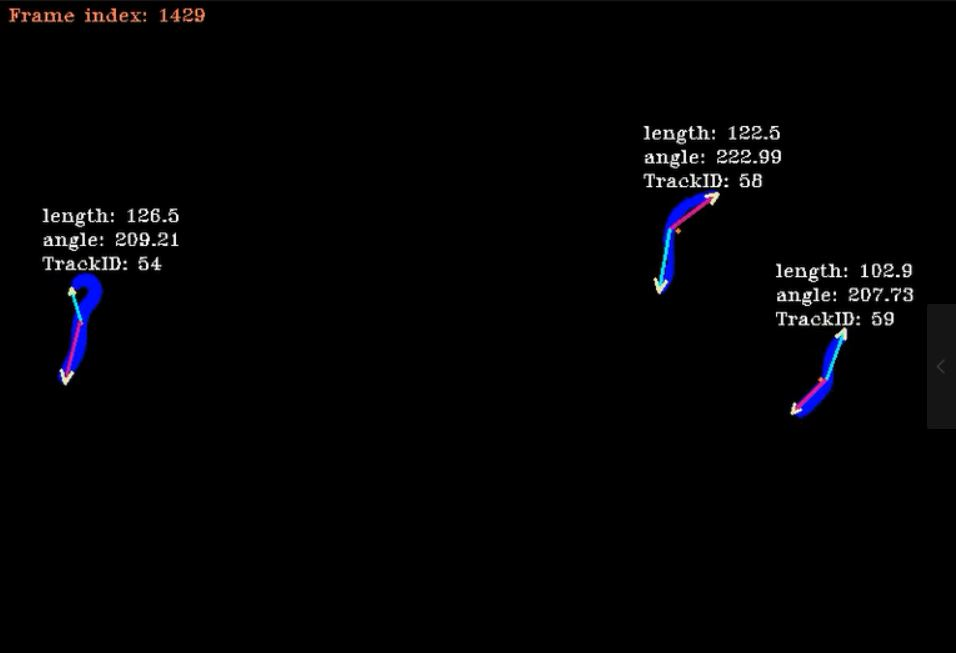
\includegraphics[width=9cm]{figure/chap5/tracking.jpg}
	  \bicaption[这里将出现在插图索引中]
		{跟踪的结果}
		{The tracking result}
	  \label{fig:track}
	\end{figure}
	矩阵中$d_{ij}$表示当前帧中的第i个轮廓的重心到上一帧中第j个轮廓的重心之间的距离。通过
	公式\ref{eq:min}可以得到相邻两帧图像中线虫轮廓之间的对应关系。即如果相邻两帧图像中两个
	轮廓重心之间的距离最短,则可以认为是同一个线虫。
		\begin{equation}
        index(i)=\mathop{\arg\min}_{j} d_{ij}\label{eq:min}
		\end{equation}
	但事实上由于轮廓分割的不完美以及图像噪声的影响
	,这一策略往往会失效。因此,通过最近邻搜索的方式来实现线虫的跟踪要满足以下的约束条件,当这两个
	条件之一不满足时,则认为跟踪丢失,此时应该分配一个新的trackID给当前的轮廓。算法\ref{algo:worm_track}
	是描述了线虫跟踪算法的实现思路。图\ref{fig:track}表示跟踪的结果。
	
	\begin{itemize}
	  \item 相邻两帧图像中同一只线虫的轮廓面积的相对变化应该小于一个阈值。
	  \item 根据线虫运动的最大速度,同一只线虫在相邻两帧图像中轮廓的重心之间的距离应该小于一个阈值。
	\end{itemize}

\begin{algorithm}
\caption{跟踪初始化程序}
\label{algo:initial_track}
\begin{algorithmic}[1]
	\Require $Worm\_data$双重列表,$Worm\_data[i][j]$表示第$i$帧图像中第$j$只线虫。
	\Ensure 输出$trackID$
	\Function {Initiate\_tracking}{$Worm\_data$}
		\State $FirstFrame\_WormData \gets Worm\_data[0]$
		\For{$i = 0 \to FirstFrame\_WormData.length-1$}
			\State $cur\_worm \gets FirstFrame\_WormData[i]$
			\State $cur\_worm.trackID \gets GetNewTrackID()$
		\EndFor
\EndFunction
\end{algorithmic}
\end{algorithm}

\begin{algorithm}[H]
\caption{线虫跟踪程序}
\label{algo:worm_track}
\begin{algorithmic}[1]
	\Require $Worm\_data$双重列表,$Worm\_data[i][j]$表示第$i$帧图像中第$j$只线虫。
	\Ensure 输出$trackID$
	\Function {Worm\_tracking}{$Worm\_data$}
		\State $Initiate\_tracking(Worm\_data)$
		\For{$frame_index = 1 \to Worm\_Data.length-1$}
			\State $PreFrame\_WormData \gets Worm\_Data[frame_index-1] $
			\For{$worm\_index =0 \to Worm\_Data[frame_index].length-1$}
% \algstore{WormTracking}
% \end{algorithmic}
% \end{algorithm}
% \begin{algorithm}[H]
% \begin{algorithmic}[1]
% \algrestore{WormTracking}
		
				\State $cur\_worm \gets Worm\_Data[frame\_index][worm\_index]$
				\State $dist\_array \gets Compute\_distance(cur\_worm,PreFrame\_WormData)$
				\State $min\_index \gets Get\_min\_index(dist\_array)$
				\State $Nearest\_worm \gets PreFrame\_WormData[min\_index]$
				\If{$\small{\frac{|Nearest\_worm.Area-cur\_worm.Area|}{Nearest\_worm.Area}<\delta \quad \text{and}  \quad dist\_array[min\_index]< \sigma}$}
					\State $cur\_worm.trackID \gets Nearest\_worm.trackID$
				\Else
					\State $cur\_worm.trackID \gets GetNewTrackID( )$
				\EndIf
			\EndFor
		\EndFor
\EndFunction
\end{algorithmic}
\end{algorithm}
\section{线虫的特征提取}
	线虫从头部到尾部两边近似等距的分布着23-24块肌肉,其头部和尾部各占其总长度的$1/6$。因此线虫
	身体的自由度为24。当用轮廓来描述线虫的形态时,在其轮廓上采样49个点足以描述线虫所有形态。
	当对线虫进行特征计算时(如:计算线虫摆动频率和运动速度等),通常是利用线虫轮廓中间的脊线进行计算。
	因此需要提取线虫轮廓的中线然后采样24个点用于特征计算。下面将首先对线虫轮廓中间脊线提取算法进行介绍,
	然后介绍线虫摆动频率的估计以及运动速度的计算。
\subsection{线虫轮廓中间脊线提取}
	在得到线虫的轮廓后,将轮廓上的坐标按顺时针排列即可得到一个坐标点的循环列表。将轮廓周长的$1/48$作为一个单位边,
	在轮廓上的任意一点其两边都可以找到一个单位边长度的相邻点,这三点所成角的补角的倒数与该点的曲率成正比,因此
	可以用于近似曲率的计算。由于其头部和尾部的变换往往比身体的其他部分要尖锐,所以如果将像素索引作为横坐标曲率作为
	纵坐标,则这条曲线上将会出现两个波峰如图\ref{fig:qulv}所示,分别对应线虫的头部和尾部。由此便可定位到线虫的头部和尾部,另外线虫的头部
	曲率一般小于尾部的曲率,两个波峰中比较低的波峰对应的横坐标为线虫头部的坐标,另一个波峰对应线虫尾部的坐标。
	线虫头部和尾部将线虫轮廓分为两边。在其中一条边上找到所有距离另一条边最近的对应点。两条边上两对应点的中点构成线虫的
	中间脊线,线虫轮廓中间脊线的长度定义为线虫的体长。
	\begin{figure}[h]
	  \centering
	  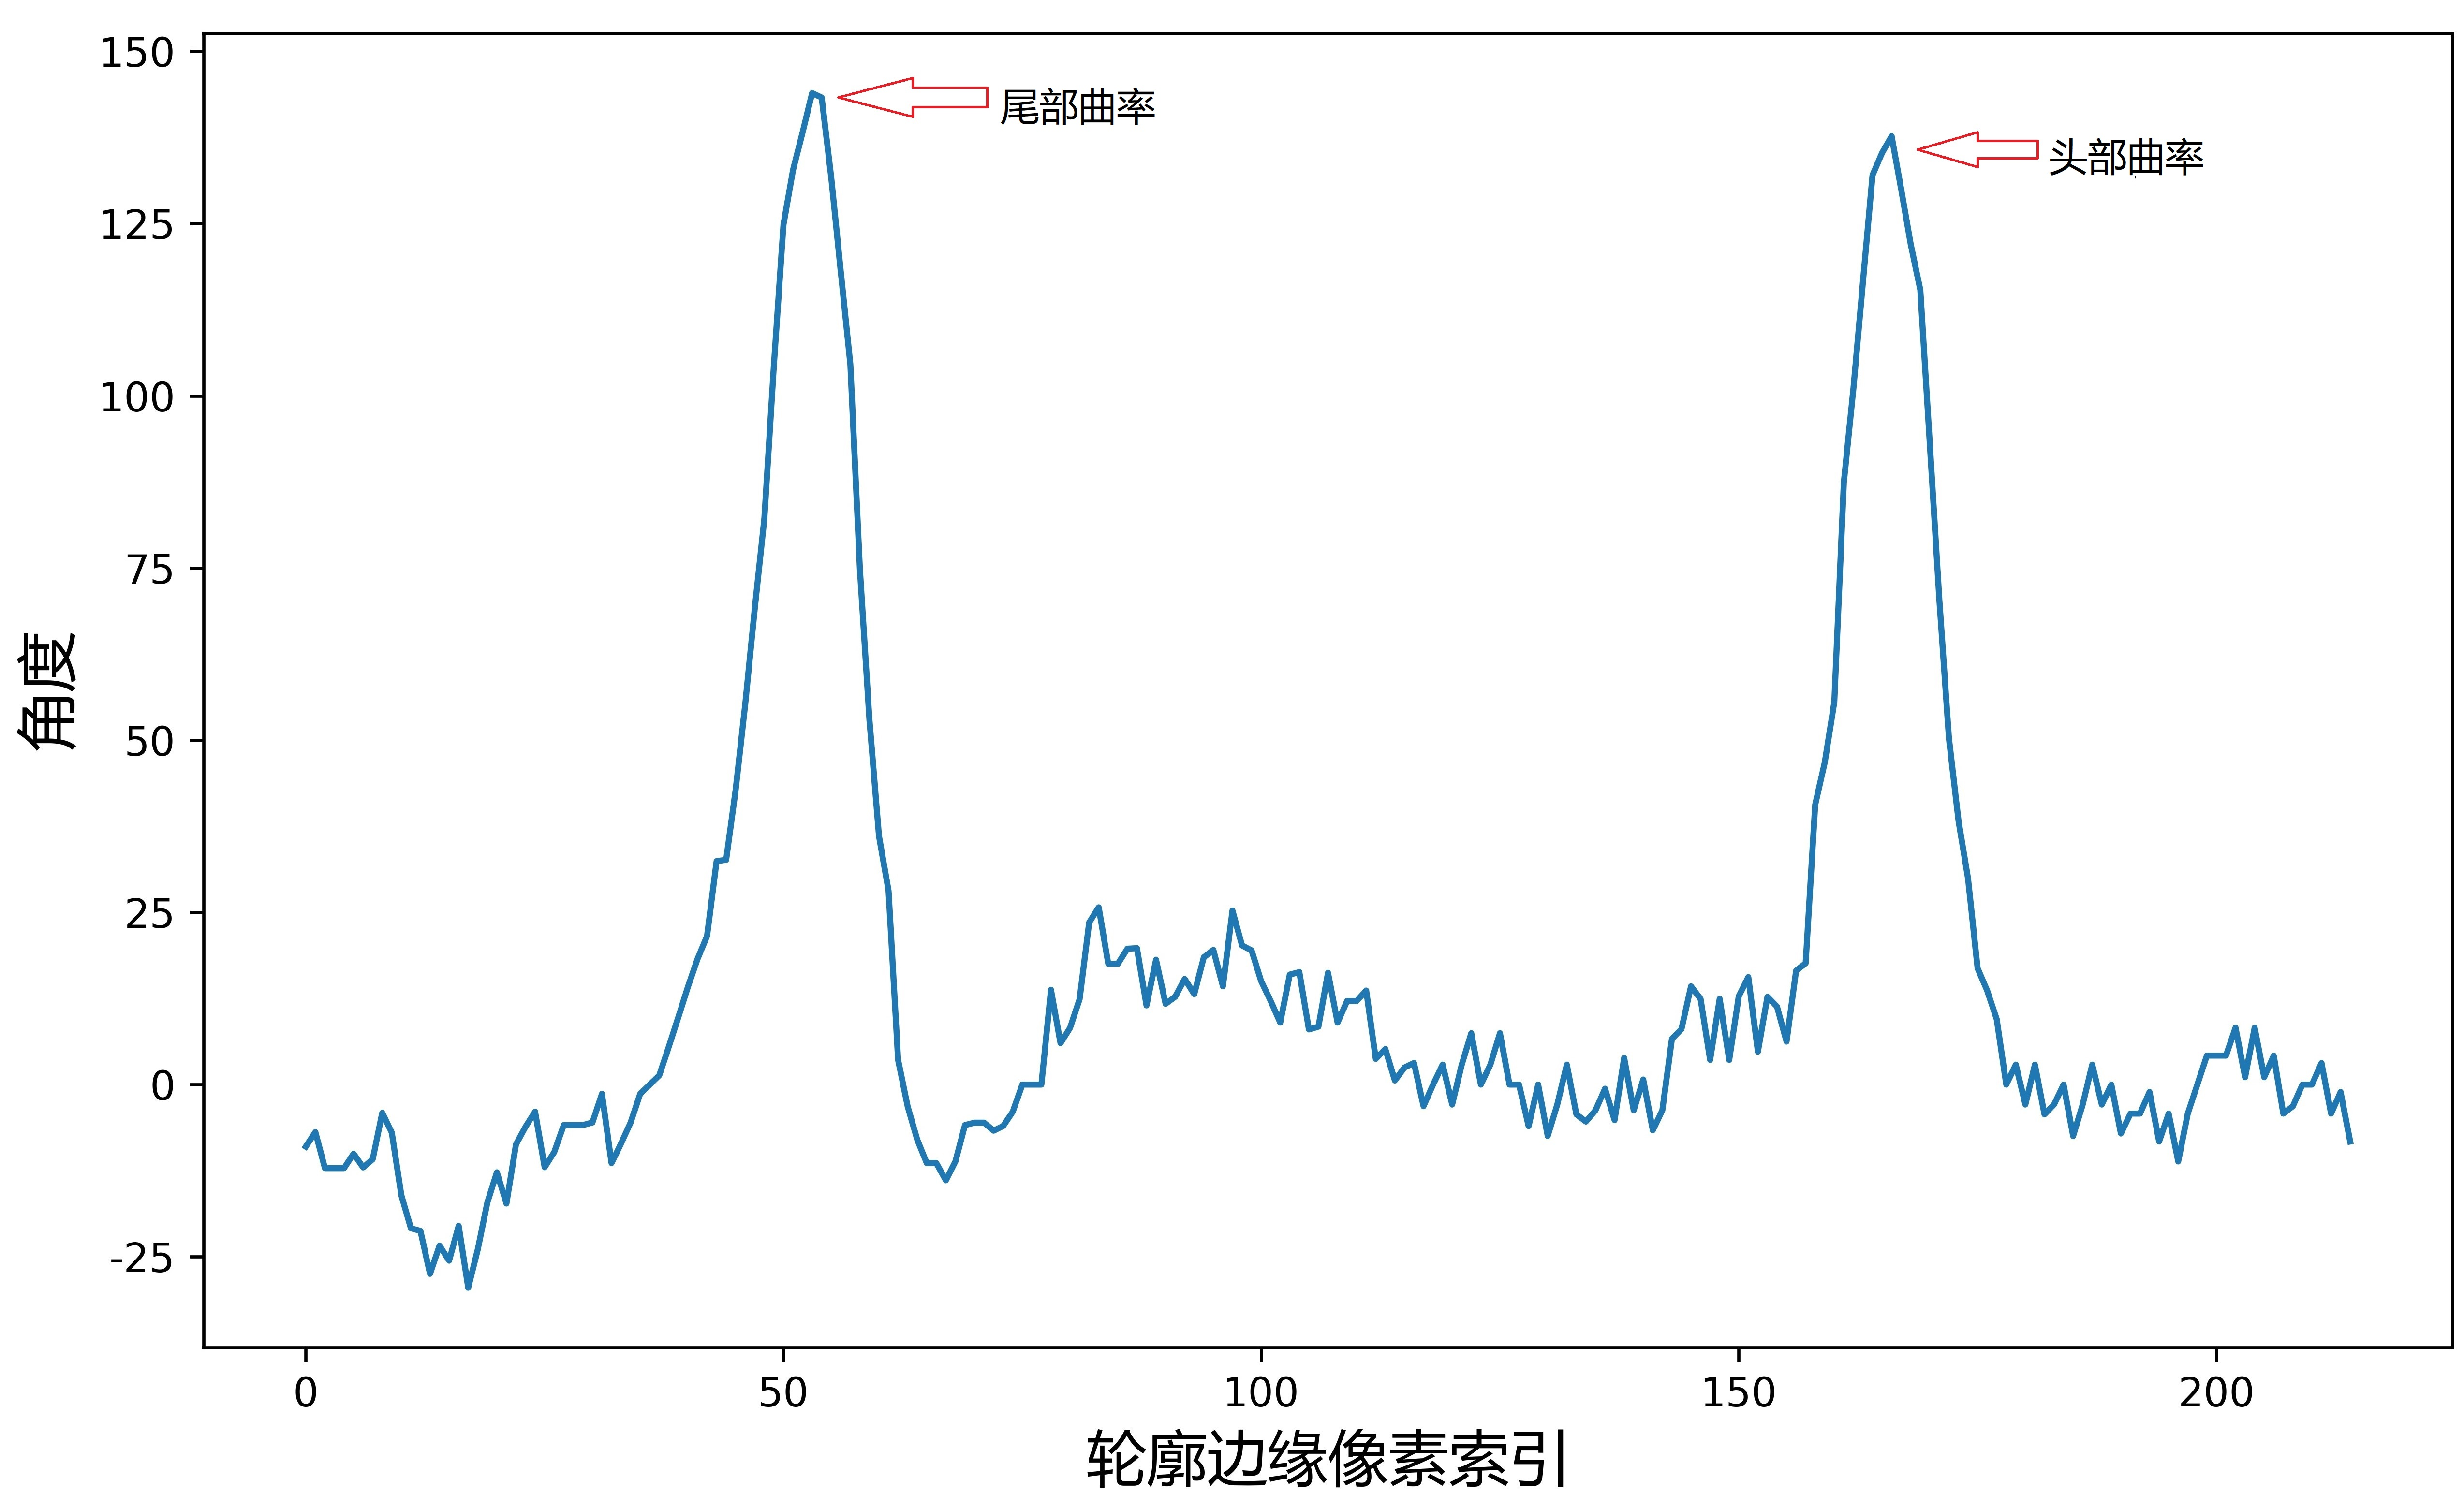
\includegraphics[width=14cm]{figure/chap5/cuvature.jpg}
	  \bicaption[这里将出现在插图索引中]
		{轮廓曲率的变化}
		{Change in contour curvature}
	  \label{fig:qulv}
	\end{figure}
\subsection{身体弯曲角度的计算以及摆动频率的估计}
	在很多毒理实验中,线虫的摆动频率经常作为一个重要的生理指标用于表征线虫的活跃程度\cite{Wang2008Assessment}。
	为了计算线虫的摆动频率, 我们定义一个衡量身体弯曲程度的夹角,由线虫头部、尾部和轮廓脊线的中点三点所成角定义为
	身体弯曲角如图\ref{fig:track}所示。线虫在爬行和游动的过程中,身体弯曲角会在$180^\circ$C左右振荡如图\ref{fig:angle},
	振荡的频率定义为线虫摆动的频率。在时刻$t_0$,对区间$(t_0-\Delta t,t_0+\Delta t)$中弯曲角信号做FFT变换,假设其幅度最大值对应的横坐标
	为n,则线虫在$t$时刻的瞬时摆动频率由公式\ref{eq:freq}得出,图\ref{fig:freq}表示线虫摆动频率随时间的变换。
	\begin{equation}
        f=\frac{frame\_rate*n}{2*\Delta t} \label{eq:freq}
	\end{equation}
		
\begin{figure}[!htp]    
% \begin{minipage}[t]{0.5\linewidth}%设定图片下字的宽度,在此基础尽量满足图片的长宽    
	\centering    
	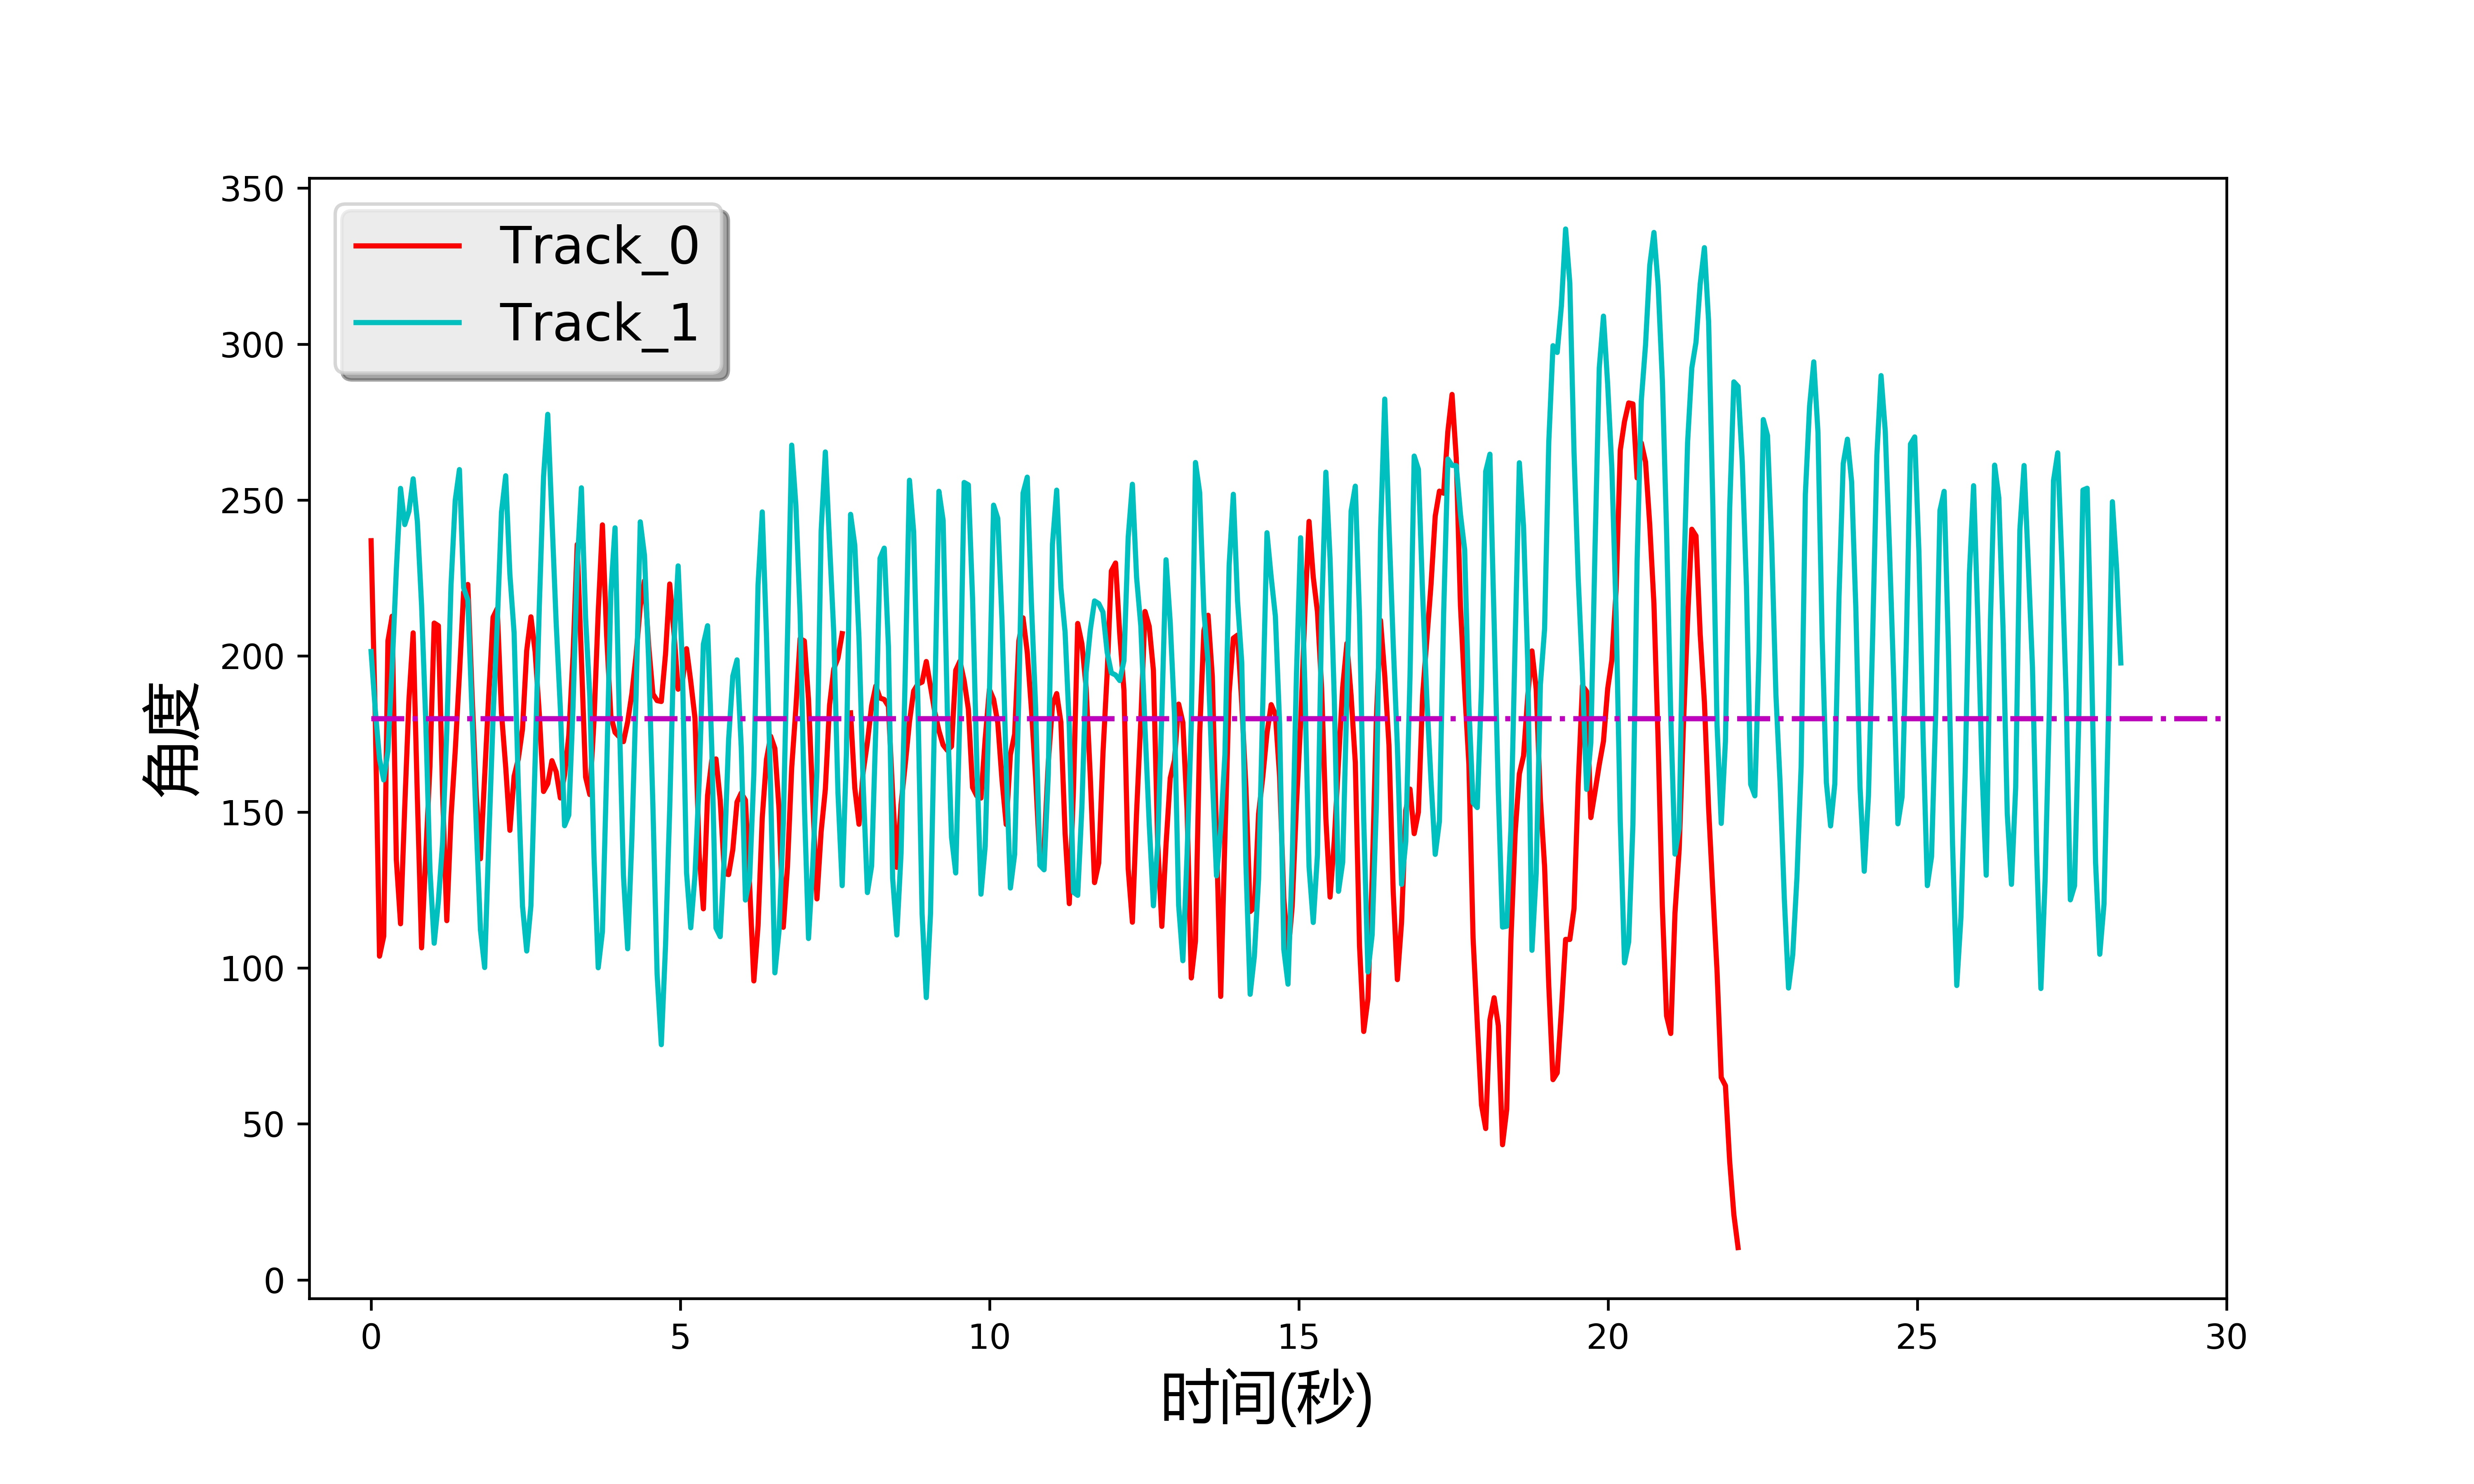
\includegraphics[width=1\linewidth]{figure/chap3/angle.jpg}    
	% \caption*{(a) 弯曲角的变化}%加*可以去掉默认前缀,作为图片单独的说明    
	% \label{fig:angle}    
% \end{minipage}    
% \begin{minipage}[t]{0.5\linewidth}%需要几张添加即可,注意设定合适的linewidth    
	% \centering    
	% 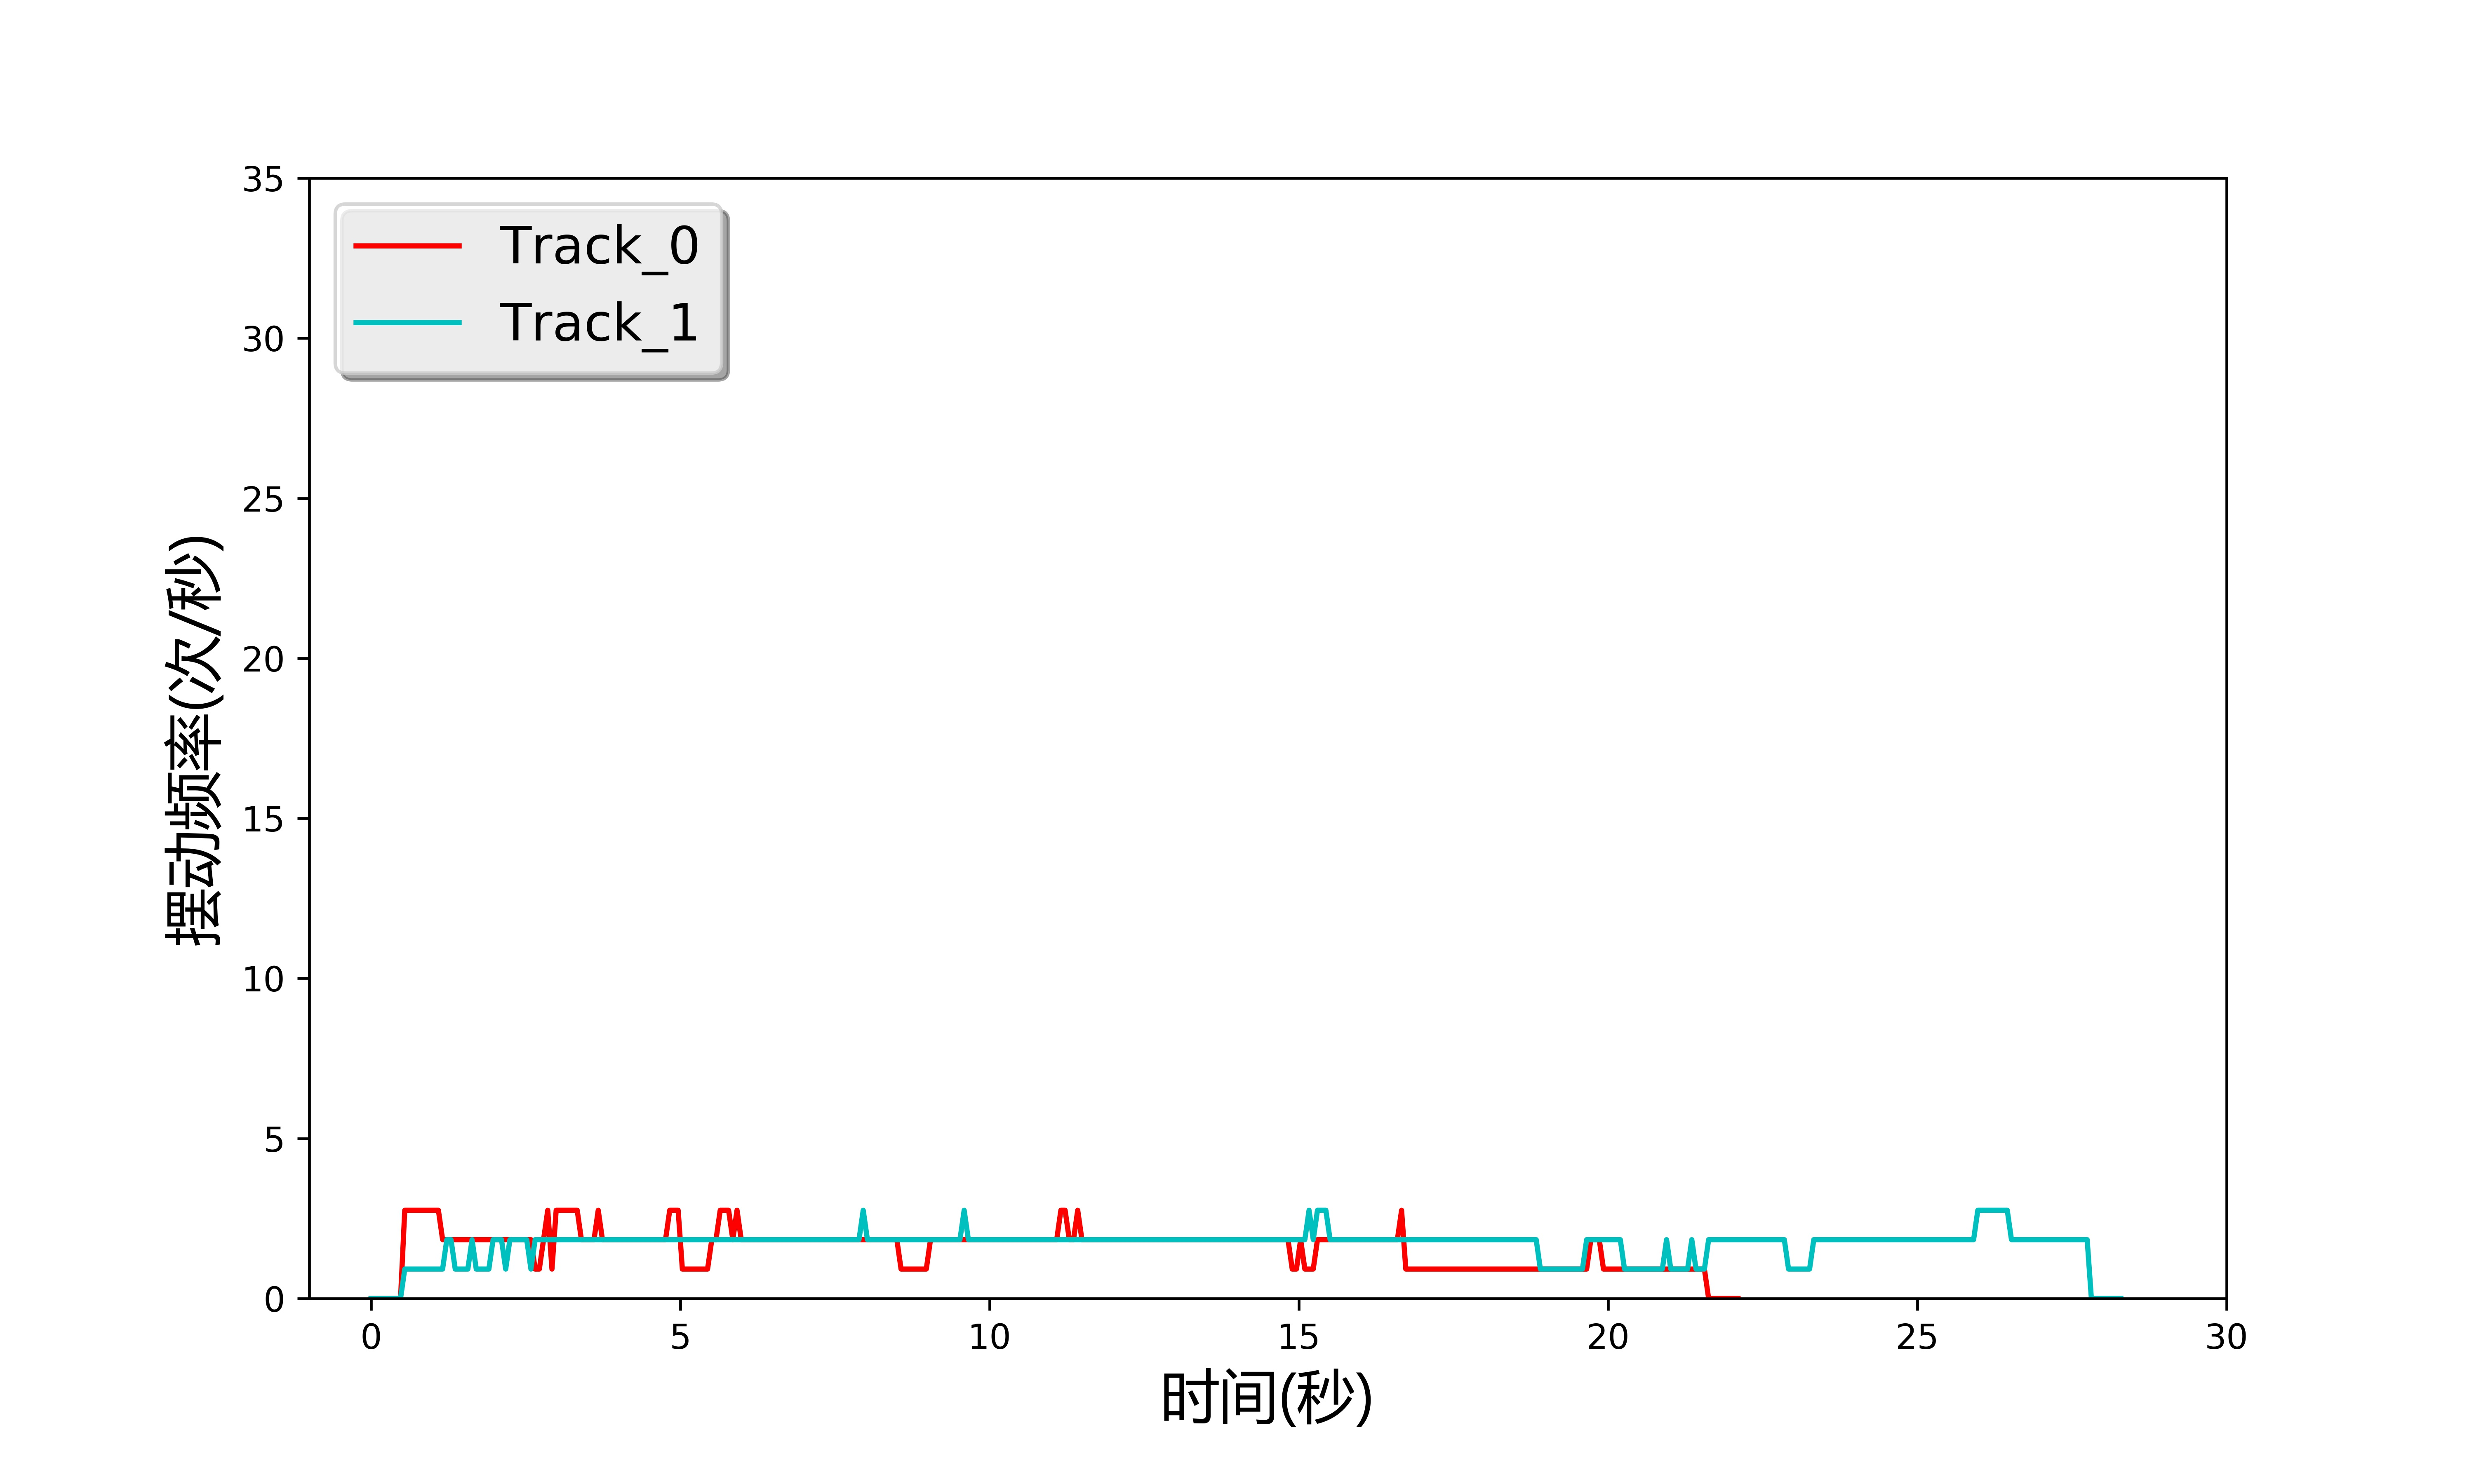
\includegraphics[width=1\linewidth]{figure/chap3/freq.jpg}    
	% \caption*{(b) 摆动频率的变化}
	% \label{fig:freq}
% \end{minipage}
\bicaption{线虫弯曲角度和摆动频率的变换}{An EPS and PDF demo with subcaptionbox}%n张图片共享的说明
\end{figure}
\section{线虫的氧化急性应激实验}
	氧化应激(Oxidative Stress,OS)指生物体氧化与抗氧化作用的失衡,当生物体被内外环境中
	存在有害化合物刺激时,其体内所产生的活性氮自由基和活性氧自由基将会导致细胞或者组织发生生理和
	病理反应。过氧化氢($H_2O_2$)溶液作为一种强氧化剂经常被用于线虫的氧化应激实验中。本文
	将野生型N2秀丽隐杆线虫的L1期幼虫作为研究对象,通过本文前面介绍的软硬件平台,研究不同线性
	浓度梯度的双氧水溶液对L1期幼虫活性的影响。
\subsection{线虫的同步化}
	为了得到处于同一发育阶段的幼虫需要对线虫进行同步化处理,首先用经过高压灭菌的M9缓冲液将NGM平板上
	混合发育期的线虫冲洗到1.5ml的离心管中,离心后去掉上清液,加入碱裂解液(体积比为1:2的5N NaOH溶液和
	5\%NaClO溶液,现配),当线虫全被腐蚀时,液体将变得清澈。再经过离心处理,去掉上层碱裂解液加入M9
	缓冲液,离心洗涤1到2次。去掉上层缓冲液并用吸管将线虫卵接种到NGM平板上,至此便完成了同步化操作,等
	线虫卵孵化便得到同步化的个体。
\subsection{线性梯度稀释芯片的操作}
	图\ref{fig:sysdevice}是实验硬件部分连接示意图,芯片上所有的阀门控制和进样控制均由Arduino单片机
	通过uln2803集成芯片控制多路电磁阀实现。将含有L1期线虫的溶液离心去上清得到线虫浓缩液,
	然后用移液枪加入0.25\%的琼脂糖溶液作为线虫助悬剂。打开6号阀门,
	采用压力进样的方式将线虫溶液从4号进样口打入第三列腔室。
	打开4号阀门用压力进样的方式将水从3号进样口打入第二列腔室。
	然后打开2号阀门用压力进样的方式将30mM的过氧化氢溶液从2号进样口打入第一列腔室。
	然后关闭2号、4号和6号阀门,打开1号、3号、5号和7号阀门,
	并在一号进样口施加一个周期性的气压。通过振荡的方式使前三列腔室中的液体充分混合。
	最后通过进样口1将混合好的液体打入第四列腔室,根据芯片腔室的尺寸设计,可以计算出混合后各腔室的过氧化氢溶液的浓度从上至小依次为:
	18mM、16mM、14mM、12mM、10mM、8mM、6mM、4mM、2mM。并用CCD相机每隔10分钟采集线虫在9个腔室中的运动视频。
	\begin{figure}[h]
	  \centering
	  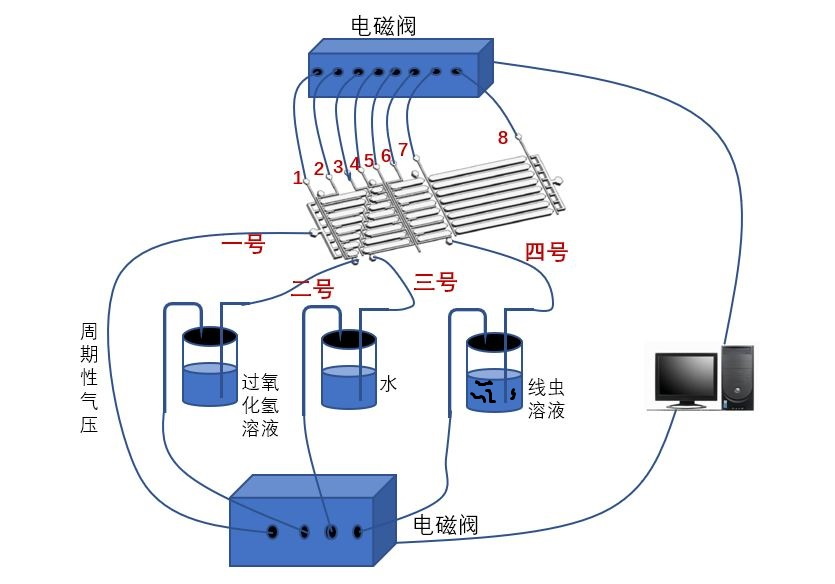
\includegraphics[width=12cm]{figure/chap5/hardware.jpg}
	  \bicaption[这里将出现在插图索引中]
		{实验系统装置示意图}
		{Change in contour curvature}
	  \label{fig:sysdevice}
	\end{figure}
\subsection{秀丽隐杆线虫急性氧化应激实验结果}
	通过本文提出的线虫轮廓分割、解析、跟踪及特征提取算法对每个腔室的各个时刻的视频进行分析并提取摆动频率特征,
	图\ref{fig:res}为了各腔室中线虫的平均摆动频率随时间的变化,可以看出随着过氧化氢溶液浓度的升高,线虫的摆动频率下降,
	且在同一浓度下,线虫的摆动频率随着时间而下降。为验证芯片实验的准确性,我们也在96孔板上手动稀释形成上述浓度后,
	通过对各个时间点线虫平均摆动频率的统计,实验结果表明96孔板实验和微流控芯片结果一致。但是相比96孔板实验,
	我们的微流控芯片平台在试剂消耗、自动分析等上面都体现了较大的优势。
	
	\begin{figure}[h]
	  \centering
	  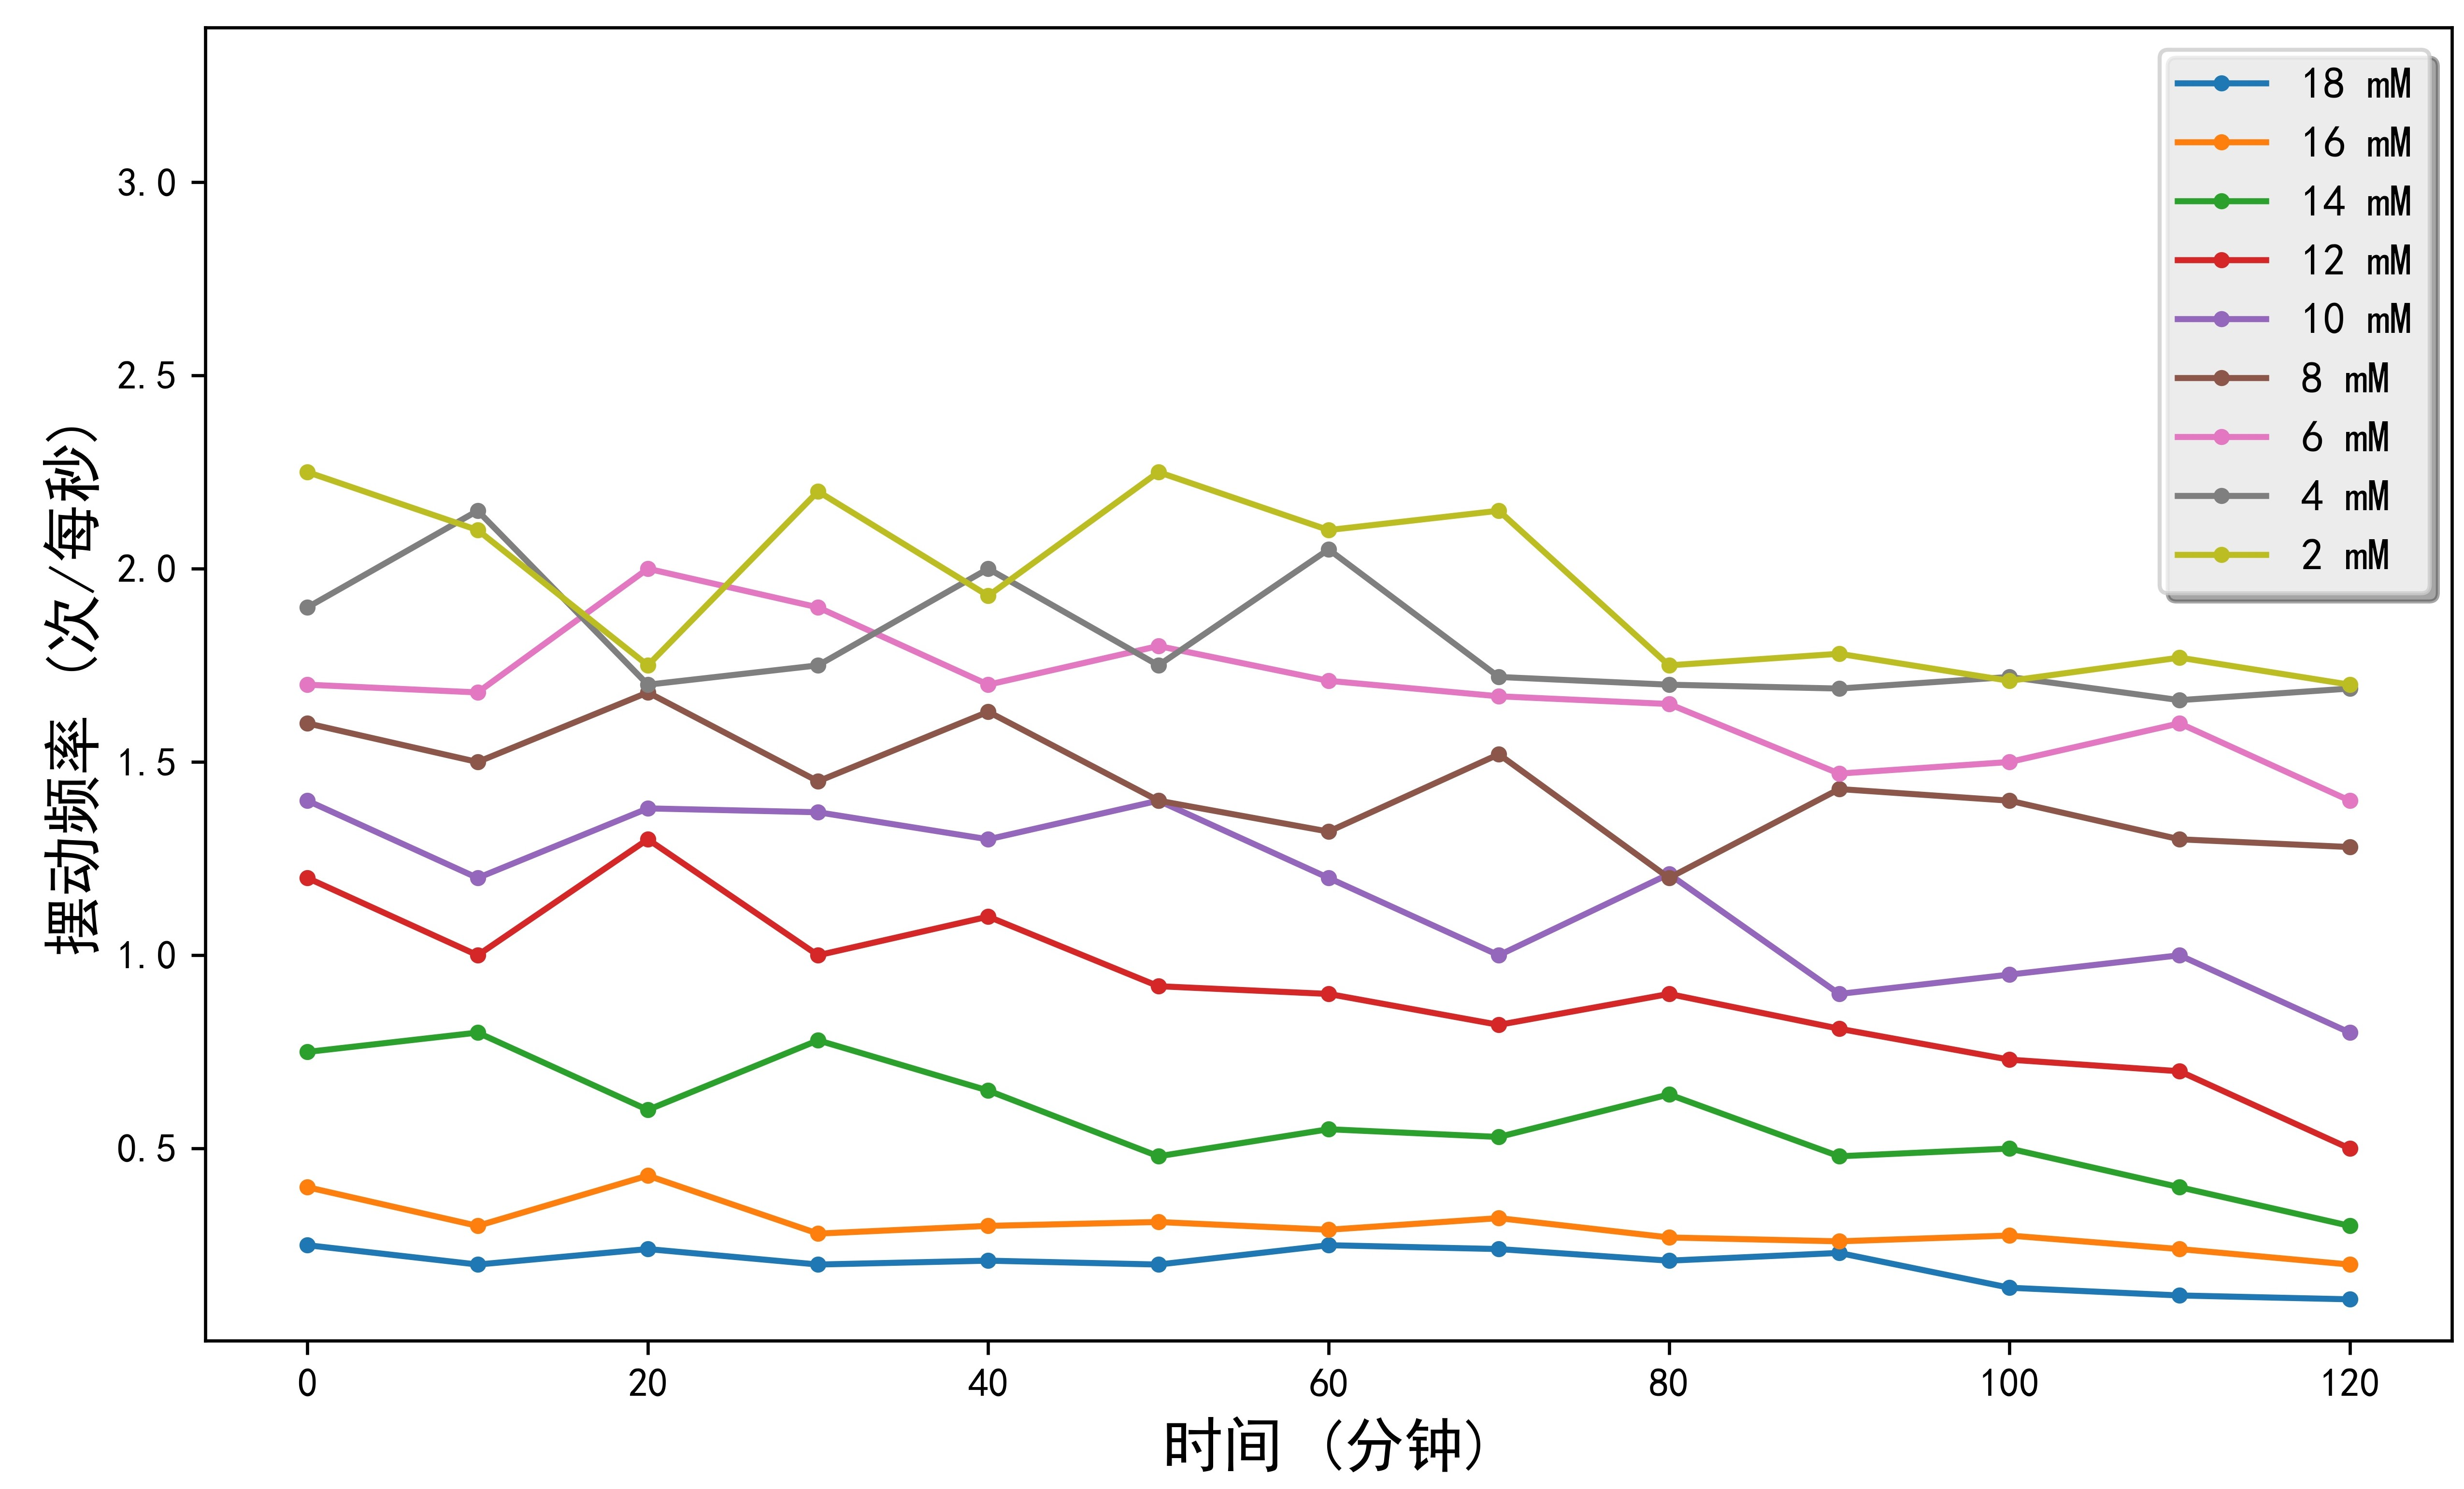
\includegraphics[width=10cm]{figure/chap5/res.jpg}
	  \bicaption[这里将出现在插图索引中]
		{各腔室中线虫平均摆动频率随时间的变化}
		{Change in contour curvature}
	  \label{fig:res}
	\end{figure}
\section{本章小结}